\begin{frame}{ЭПР-парадокс}
 \begin{columns}
   \column{0.4\textwidth}
   \begin{figure}
     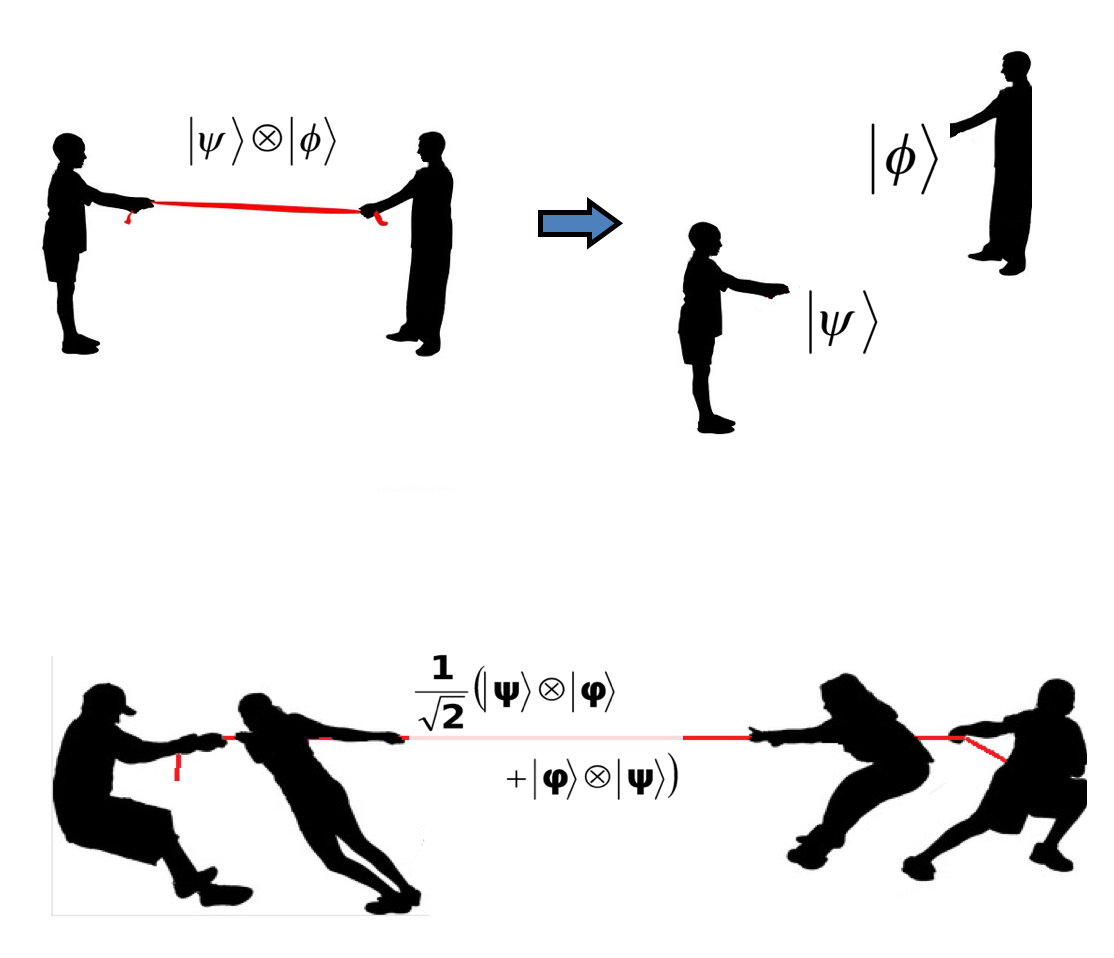
\includegraphics[width=\textwidth]{bi-entanglement.png}
   \end{figure}

   \column{0.5\textwidth}
   \begin{block}{}
     Работа Эйнштейна—Подольского-Розена\footnote[frame]{A. Einstein, B. Podolsky, and N. Rosen \textit{Phys. Rev.} \textbf{47}, 777 (1935)}
     указывала на неполноту квантовой механики с помощью мысленного эксперимента,
     заключающегося в измерении параметров микрообъекта косвенным образом,
     без непосредственного воздействия на этот объект.
   \end{block}
   \begin{block}{}
      В 2008 году был проведен эксперимент\footnote[frame]{T. Scheidl et al. \textit{PNAS} \textbf{107}, 46, 19708-19713 (2010)},
      который подтвердил нелокальный\footnote[frame]{J.S. Bell \textit{Physics Physique Fizika} \textbf{1}, 195 (1964)}
      характер квантовой теории.
   \end{block}
 \end{columns}
\end{frame}
\note{
  В 35 году была опубликована ЭПР.
  Она указвывала на ...слайд...

  Джон Стюарт Белл предложил эксперимент который ...

  Первый эксперимент был проведен Джоном Клаузером в 1972 (википедия).
  Второй первый эксперимент был проведен Аленом Аспе в 70е.
  (Alain Aspect Phys. Rev. D 14, 1944 – Published 15 October 1976)
  И затем было еще много экспериментов.

  В 2010 году Джон Клаузер, Ален Аспе и Антон Цайлингер стали лауреатами премии Вольфа по физике «за фундаментальный концептуальный и экспериментальный вклад в основы квантовой физики, в частности за серию возрастающих по сложности проверок неравенств Белла (или расширенных версий этих неравенств) с использованием запутанных квантовых состояний»
}

\begin{frame}{Квантовые технологии}
  \begin{columns}
   \column{0.6\textwidth}
   \begin{figure}
     \begin{subfigure}[t]{0.33\textwidth}
       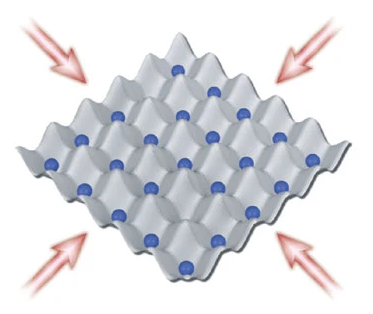
\includegraphics[width=\textwidth]{ultracold-atoms.png}
       %\captionsetup{labelformat=empty}
       \caption{Ultracold atoms}
       \label{fig:ultracold-atoms}
     \end{subfigure}
     \begin{subfigure}[t]{0.33\textwidth}
       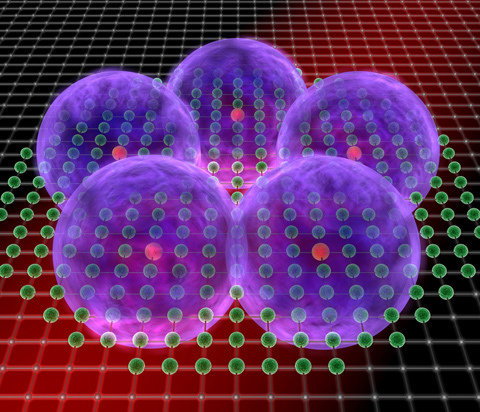
\includegraphics[width=\textwidth]{ridberg-atoms.png}
       %\captionsetup{labelformat=empty}
       \caption{Rydberg atoms}
     \end{subfigure}
     % \vspace*{2mm}
     \vfill
     \begin{subfigure}[t]{0.33\textwidth}
       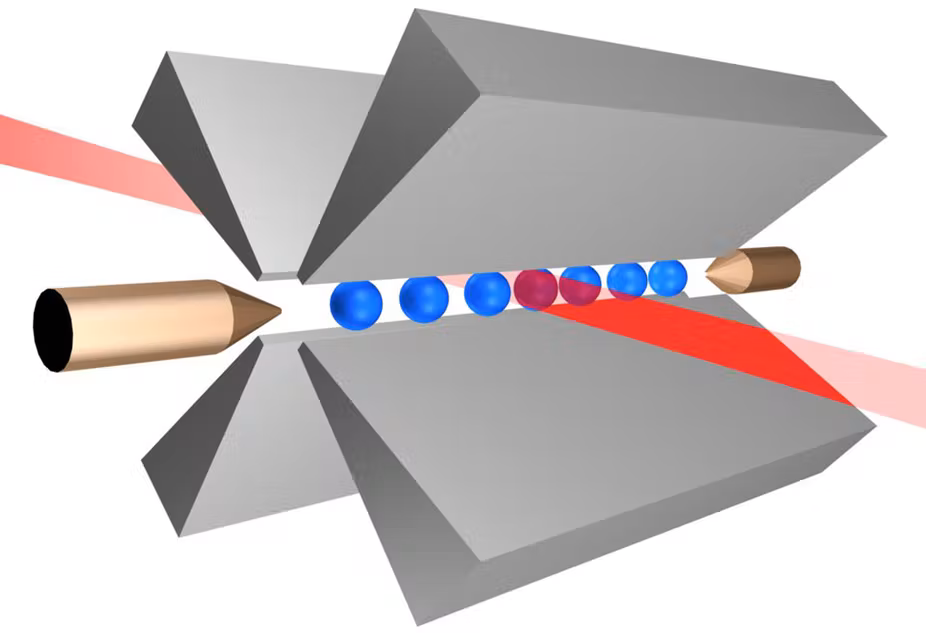
\includegraphics[width=\textwidth]{trapped-ions.png}
       %\captionsetup{labelformat=empty}
       \caption{Trapped ions}
     \end{subfigure}
     \begin{subfigure}[t]{0.33\textwidth}
       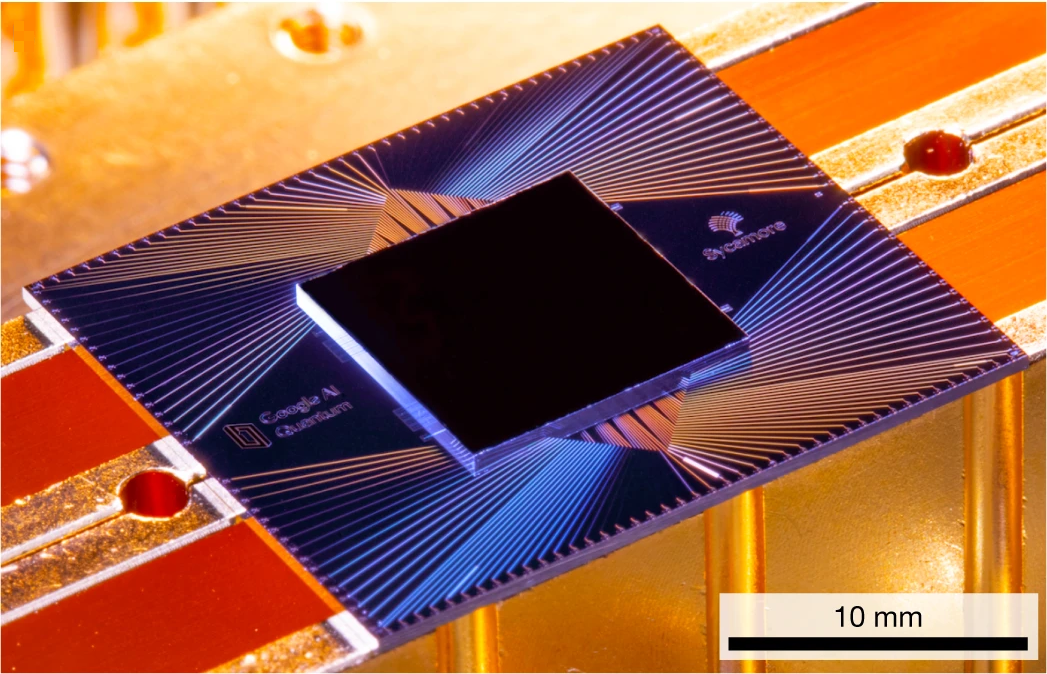
\includegraphics[width=\textwidth]{sycamore.png}
       %\captionsetup{labelformat=empty}
       \caption{SC qubits}
     \end{subfigure}
     \caption{
       Квантовые платформы.
       % (\ref{fig:ultracold-atoms})~{Bloch, I. Nature 453, 1016–1022 (2008)}
     }
   \end{figure}

   \column{0.4\textwidth}
   \begin{figure}
       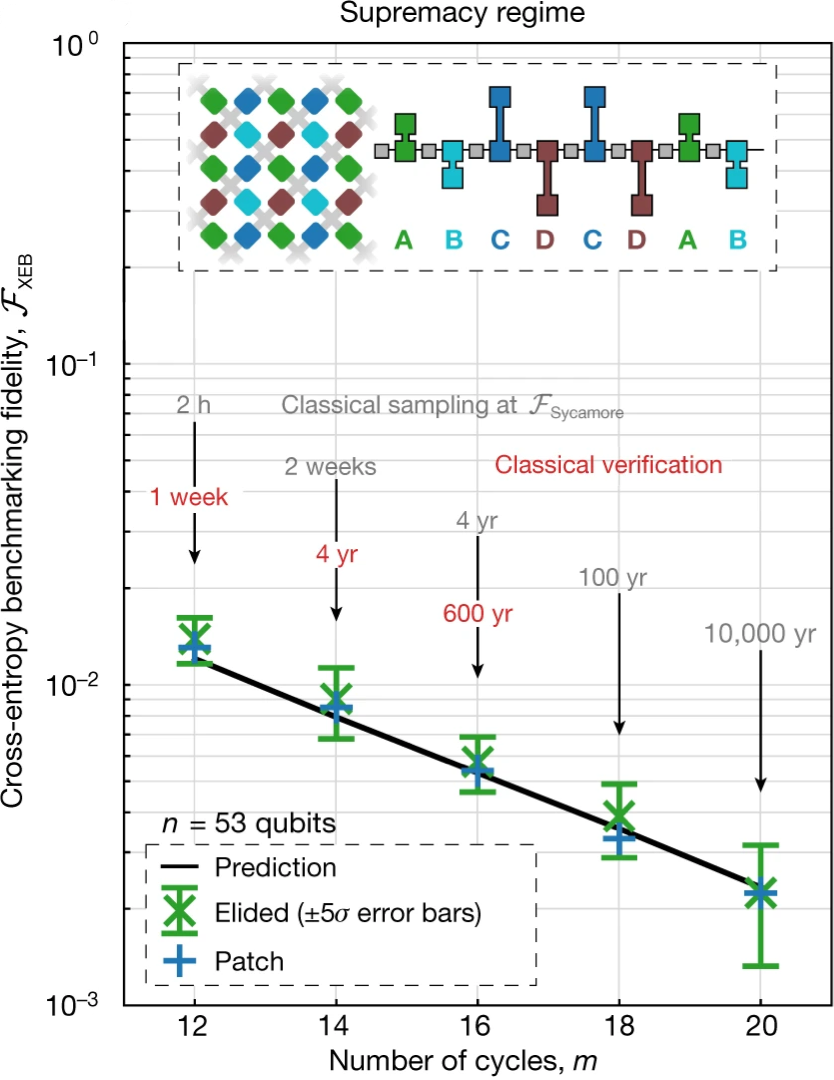
\includegraphics[width=0.8\textwidth]{sycamore-supemancy.png}
       % \captionsetup{labelformat=empty}
       \caption{
         % F. Arute et al., Nature 574, 505 (2019)
         Nature 574, 505 (2019)
       }
     \end{figure}
   \end{columns}
\end{frame}
\note{
  Активная разработка квантовых компьютеров.
  Квантовые платформы и их сравнение.

  \textbf{ЯМР}
  ЯМР был первым, но он негодится для вычислений (нет чистых состояний).
  Отлично подходит для исследований.
  Много наработок.

  Исследуется все гильбертого пространство.
  Квантовое превосходство  на программируемом сверхпроводящем процессоре.
  Запутанные состояния являются важным ресурсом в квантовых вычисления:
  Например, недавно продемонстрированное группой Мартинеса квантовое превосходство [1] на программируемом сверхпроводящем процессоре связано с понятием запутанноси
}



\begin{frame}{Бинарная запутанность}
  \begin{columns}
    \column{0.57\textwidth}
    $$
      \left| \Psi \right\rangle
      = \frac{
        \left| \uparrow\uparrow \right\rangle +
        \left| \downarrow\downarrow \right\rangle
      }{\sqrt{2}}
    $$
    \begin{block}{Критерии запутанности}
      \begin{itemize}
        \item Энтропия фон-Неймана \\
          {\footnotesize C.H.Bennett et al. \textit{Phys. Rev. A} \textbf{54}, 3824 (1996)}
        \item Критерий Вуттеса \\
          {\footnotesize W.K. Wootters, \textit{Phys. Rev. Lett.} \textbf{80}, 2245 (1998)}
        \item Мера Шмидта \\
          {\footnotesize Eisert J. and Briegel H. J. \textit{Phys. Rev. A} \textbf{64}, 022306 (2001)}
        \item ...
      \end{itemize}
    \end{block}

    %\begin{example}
    %  Запутанность в нитрозильном комплексе железа (НКЖ)\footnote[frame]{S. M. Aldoshin, E. B. Feldman, and M. A. Yurishchev, \textit{JETP} \textbf{107}, 5, 804–811 (2008)}.
    %\end{example}

    \column{0.4\textwidth}
    %\vspace{-2mm}
    \begin{figure}
      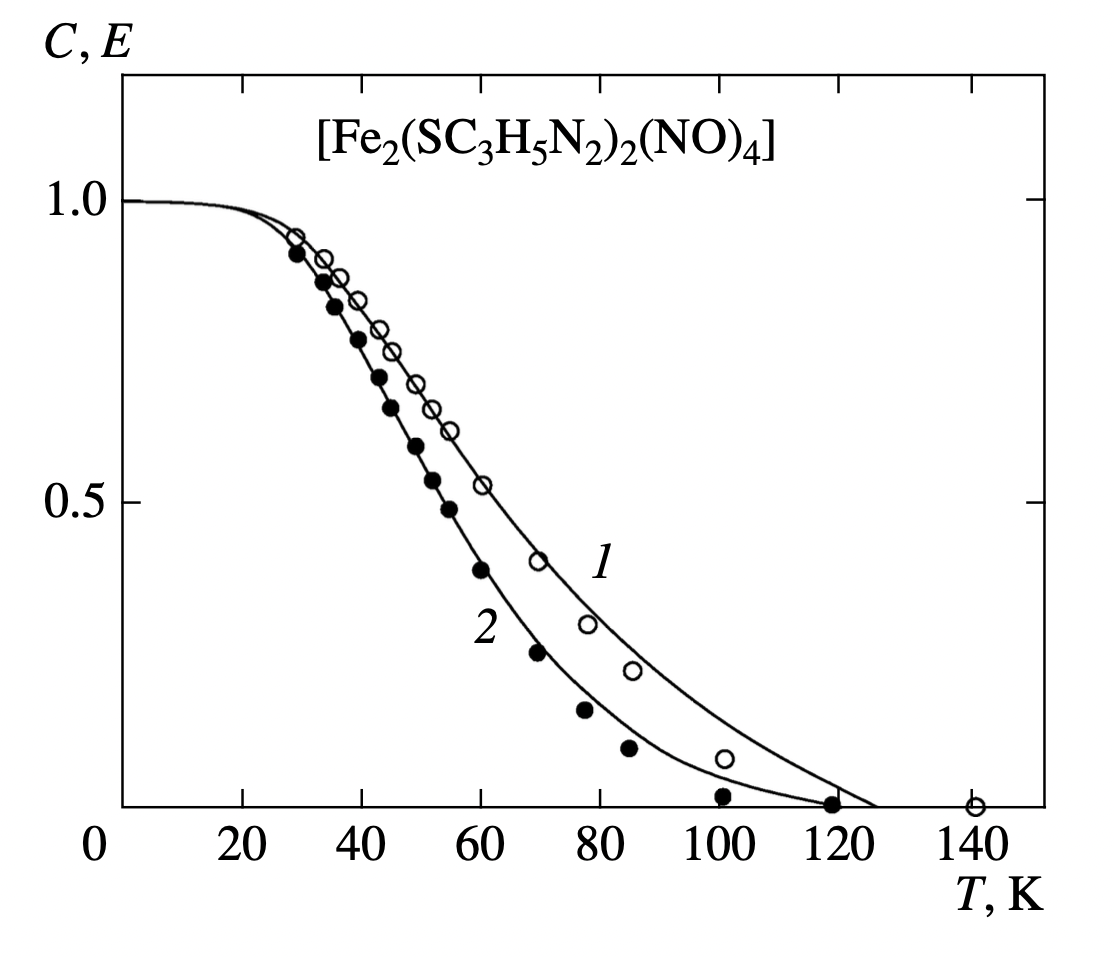
\includegraphics[width=\textwidth]{bi-entanglement-jetp2008.png}
      \captionsetup{skip=-2mm}
      \caption{Температурная зависимость согласованности (1) и запутанности (2) для нитрозильного комплекса железа\footnote[frame]{S. M. Aldoshin, E. B. Feldman, and M. A. Yurishchev, \textit{JETP} \textbf{107}, 5, 804–811 (2008)}.}
    \end{figure}
  \end{columns}
\end{frame}
\note{
  На слайде приведен пример cостояния с бинарной запутанностью.
  Измерение одной частицы определяет состояние второй.

  Определения таких состояний не тривиальная задача.
  В действительности, чтобы показать, что состояние запутанно нужно еще угадать с проективными измерениями,
  так как в произвольном базисе нельзя установить факт наличия запутанности.

  Эта задача уже хорошо разработана
  и было предложено множество критериев для выявления таких корреляций.
  например  мера Шмидта, согласованность Вуттерса, энропия фон-Неймана.


  Этот эффект хорошо изучен экспериментально, в качестве примера
  на слайде приведен результат из работы нашего института.
  Это температурная зависимость величины запутанности
  подсчитаной на основе согласованности в нитрозильном комплексе железа.
  Линии это теоретический расчет, точки это эксперимент.

  Такие результаты удается получит благодаря тому, что согласованность
  Вуттерса связана с магнитной восприимчивостью атиферомагнитного димера.
}



\begin{frame}{Цели и задачи}
  \textbf{Целью данной работы} является теоретическое исследование многочастичной запутанности в системах с большим количеством частиц $(>200)$ в рамках МК спектроскопии ЯМР,
а также развитие методов экспериментального измерения квантовых информационных величин.
\end{frame}
